% This file was created with tikzplotlib v0.9.12.
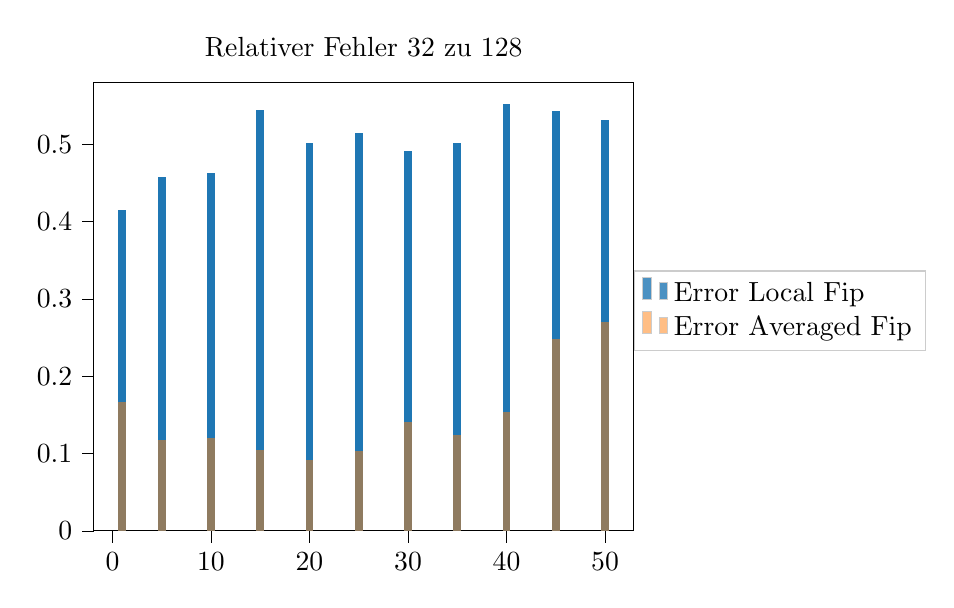
\begin{tikzpicture}

\definecolor{color0}{rgb}{0.12156862745098,0.466666666666667,0.705882352941177}
\definecolor{color1}{rgb}{1,0.498039215686275,0.0549019607843137}

\begin{axis}[
legend cell align={left},
legend style={
  fill opacity=0.8,
  draw opacity=1,
  text opacity=1,
  at={(1,0.4)},
  anchor=south west,
  draw=white!80!black
},
tick align=outside,
tick pos=left,
title={Relativer Fehler 32 zu 128},
x grid style={white!69.0196078431373!black},
xmin=-1.89, xmax=52.89,
xtick style={color=black},
y grid style={white!69.0196078431373!black},
ymin=0, ymax=0.579925374370528,
ytick style={color=black}
]
\draw[draw=none,fill=color0] (axis cs:0.6,0) rectangle (axis cs:1.4,0.415062858240941);
\addlegendimage{ybar,ybar legend,draw=none,fill=color0}
\addlegendentry{Error Local Fip}

\draw[draw=none,fill=color0] (axis cs:4.6,0) rectangle (axis cs:5.4,0.457964217507584);
\draw[draw=none,fill=color0] (axis cs:9.6,0) rectangle (axis cs:10.4,0.462779149555444);
\draw[draw=none,fill=color0] (axis cs:14.6,0) rectangle (axis cs:15.4,0.544447033329513);
\draw[draw=none,fill=color0] (axis cs:19.6,0) rectangle (axis cs:20.4,0.501048160125471);
\draw[draw=none,fill=color0] (axis cs:24.6,0) rectangle (axis cs:25.4,0.51460839961401);
\draw[draw=none,fill=color0] (axis cs:29.6,0) rectangle (axis cs:30.4,0.490661385792495);
\draw[draw=none,fill=color0] (axis cs:34.6,0) rectangle (axis cs:35.4,0.50169494565827);
\draw[draw=none,fill=color0] (axis cs:39.6,0) rectangle (axis cs:40.4,0.552309880352884);
\draw[draw=none,fill=color0] (axis cs:44.6,0) rectangle (axis cs:45.4,0.543232722165154);
\draw[draw=none,fill=color0] (axis cs:49.6,0) rectangle (axis cs:50.4,0.531587788964543);
\draw[draw=none,fill=color1,fill opacity=0.5] (axis cs:0.6,0) rectangle (axis cs:1.4,0.167001786466406);
\addlegendimage{ybar,ybar legend,draw=none,fill=color1,fill opacity=0.5}
\addlegendentry{Error Averaged Fip}

\draw[draw=none,fill=color1,fill opacity=0.5] (axis cs:4.6,0) rectangle (axis cs:5.4,0.118084017073864);
\draw[draw=none,fill=color1,fill opacity=0.5] (axis cs:9.6,0) rectangle (axis cs:10.4,0.11967093199986);
\draw[draw=none,fill=color1,fill opacity=0.5] (axis cs:14.6,0) rectangle (axis cs:15.4,0.104402054764689);
\draw[draw=none,fill=color1,fill opacity=0.5] (axis cs:19.6,0) rectangle (axis cs:20.4,0.0911535344393767);
\draw[draw=none,fill=color1,fill opacity=0.5] (axis cs:24.6,0) rectangle (axis cs:25.4,0.102630142512145);
\draw[draw=none,fill=color1,fill opacity=0.5] (axis cs:29.6,0) rectangle (axis cs:30.4,0.140325061732502);
\draw[draw=none,fill=color1,fill opacity=0.5] (axis cs:34.6,0) rectangle (axis cs:35.4,0.124332115062361);
\draw[draw=none,fill=color1,fill opacity=0.5] (axis cs:39.6,0) rectangle (axis cs:40.4,0.153875539865767);
\draw[draw=none,fill=color1,fill opacity=0.5] (axis cs:44.6,0) rectangle (axis cs:45.4,0.24791496631234);
\draw[draw=none,fill=color1,fill opacity=0.5] (axis cs:49.6,0) rectangle (axis cs:50.4,0.269842716008983);
\end{axis}

\end{tikzpicture}
